\documentclass{standalone}
\usepackage{tikz}
\usetikzlibrary{patterns, positioning}

\begin{document}
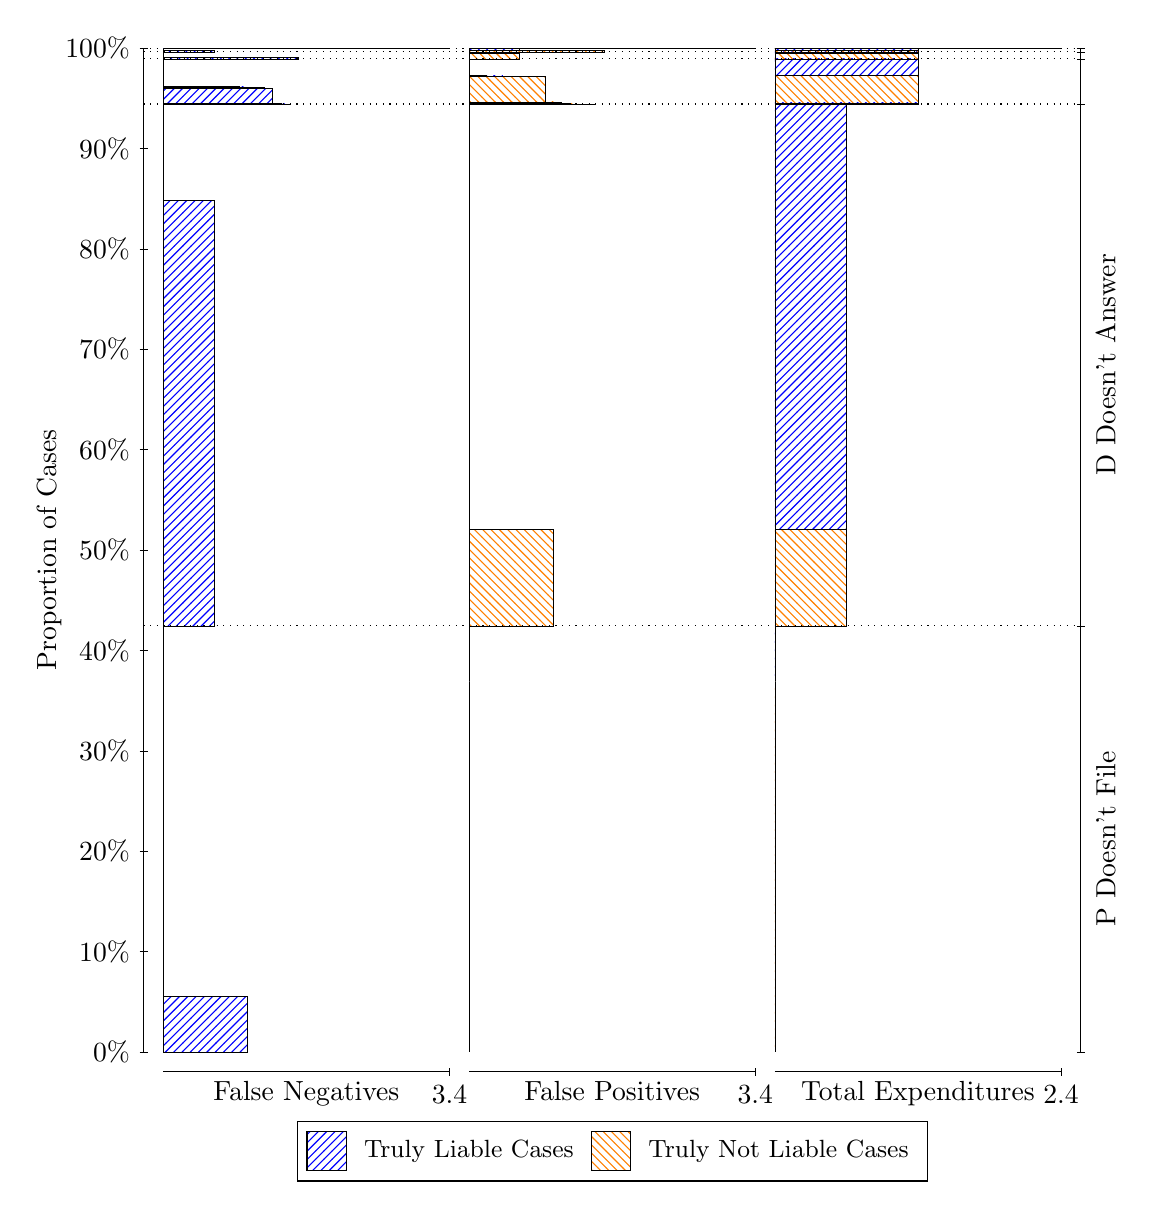
\begin{tikzpicture}
\draw[black, very thin] (1.5,1.75) -- (1.5,14.5);
\node[rotate=90, anchor=center] at (0.3, 8.125) {Proportion of Cases};
\draw[black, very thin] (1.45,1.75) -- (1.55,1.75);
\node[anchor=east] at (1.45, 1.75) {0\%};
\draw[black, very thin] (1.45,3.025) -- (1.55,3.025);
\node[anchor=east] at (1.45, 3.025) {10\%};
\draw[black, very thin] (1.45,4.3) -- (1.55,4.3);
\node[anchor=east] at (1.45, 4.3) {20\%};
\draw[black, very thin] (1.45,5.575) -- (1.55,5.575);
\node[anchor=east] at (1.45, 5.575) {30\%};
\draw[black, very thin] (1.45,6.85) -- (1.55,6.85);
\node[anchor=east] at (1.45, 6.85) {40\%};
\draw[black, very thin] (1.45,8.125) -- (1.55,8.125);
\node[anchor=east] at (1.45, 8.125) {50\%};
\draw[black, very thin] (1.45,9.4) -- (1.55,9.4);
\node[anchor=east] at (1.45, 9.4) {60\%};
\draw[black, very thin] (1.45,10.675) -- (1.55,10.675);
\node[anchor=east] at (1.45, 10.675) {70\%};
\draw[black, very thin] (1.45,11.95) -- (1.55,11.95);
\node[anchor=east] at (1.45, 11.95) {80\%};
\draw[black, very thin] (1.45,13.225) -- (1.55,13.225);
\node[anchor=east] at (1.45, 13.225) {90\%};
\draw[black, very thin] (1.45,14.5) -- (1.55,14.5);
\node[anchor=east] at (1.45, 14.5) {100\%};

\draw[black, very thin] (13.4,1.75) -- (13.4,14.5);
\draw[black, very thin] (13.35,1.75) -- (13.45,1.75);
\node[anchor=west] at (13.35, 1.75) {};
\draw[black, very thin] (13.35,7.161) -- (13.45,7.161);
\node[anchor=west] at (13.35, 7.161) {};
\draw[black, very thin] (13.35,13.789) -- (13.45,13.789);
\node[anchor=west] at (13.35, 13.789) {};
\draw[black, very thin] (13.35,14.363) -- (13.45,14.363);
\node[anchor=west] at (13.35, 14.363) {};
\draw[black, very thin] (13.35,14.451) -- (13.45,14.451);
\node[anchor=west] at (13.35, 14.451) {};
\draw[black, very thin] (13.35,14.497) -- (13.45,14.497);
\node[anchor=west] at (13.35, 14.497) {};
\draw[black, very thin] (13.35,14.499) -- (13.45,14.499);
\node[anchor=west] at (13.35, 14.499) {};
\draw[black, very thin] (13.35,14.5) -- (13.45,14.5);
\node[anchor=west] at (13.35, 14.5) {};

\draw[black, very thin, pattern color=blue, pattern=north east lines] (1.75,1.75) rectangle (2.8186,2.4582);
\draw[black, very thin, pattern color=orange, pattern=north west lines] (1.75,2.4582) rectangle (1.75,7.161);
\draw[black, very thin, pattern color=blue, pattern=north east lines] (1.75,7.161) rectangle (2.3912,12.563);
\draw[black, very thin, pattern color=orange, pattern=north west lines] (1.75,12.563) rectangle (1.75,13.789);
\draw[black, very thin, pattern color=blue, pattern=north east lines] (1.75,13.789) rectangle (3.3529,13.79);
\draw[black, very thin, pattern color=blue, pattern=north east lines] (1.75,13.79) rectangle (3.2461,13.794);
\draw[black, very thin, pattern color=blue, pattern=north east lines] (1.75,13.794) rectangle (3.1392,13.992);
\draw[black, very thin, pattern color=blue, pattern=north east lines] (1.75,13.992) rectangle (3.0324,13.997);
\draw[black, very thin, pattern color=blue, pattern=north east lines] (1.75,13.997) rectangle (2.9255,14.002);
\draw[black, very thin, pattern color=blue, pattern=north east lines] (1.75,14.002) rectangle (2.8186,14.007);
\draw[black, very thin, pattern color=blue, pattern=north east lines] (1.75,14.007) rectangle (2.7118,14.008);
\draw[black, very thin, pattern color=blue, pattern=north east lines] (1.75,14.008) rectangle (2.6049,14.008);
\draw[black, very thin, pattern color=blue, pattern=north east lines] (1.75,14.008) rectangle (2.498,14.008);
\draw[black, very thin, pattern color=orange, pattern=north west lines] (1.75,14.008) rectangle (1.75,14.363);
\draw[black, very thin, pattern color=blue, pattern=north east lines] (1.75,14.363) rectangle (3.4598,14.385);
\draw[black, very thin, pattern color=orange, pattern=north west lines] (1.75,14.385) rectangle (1.75,14.451);
\draw[black, very thin, pattern color=blue, pattern=north east lines] (1.75,14.451) rectangle (2.3912,14.474);
\draw[black, very thin, pattern color=orange, pattern=north west lines] (1.75,14.474) rectangle (1.75,14.497);
\draw[black, very thin, pattern color=blue, pattern=north east lines] (1.75,14.497) rectangle (5.3833,14.497);
\draw[black, very thin, pattern color=orange, pattern=north west lines] (1.75,14.497) rectangle (1.75,14.499);
\draw[black, very thin, pattern color=orange, pattern=north west lines] (1.75,14.499) rectangle (1.75,14.499);
\draw[black, very thin, pattern color=blue, pattern=north east lines] (1.75,14.499) rectangle (1.75,14.5);
\draw[black, very thin, pattern color=orange, pattern=north west lines] (5.6333,1.75) rectangle (5.6333,6.4528);
\draw[black, very thin, pattern color=blue, pattern=north east lines] (5.6333,6.4528) rectangle (5.6333,7.161);
\draw[black, very thin, pattern color=orange, pattern=north west lines] (5.6333,7.161) rectangle (6.702,8.3871);
\draw[black, very thin, pattern color=blue, pattern=north east lines] (5.6333,8.3871) rectangle (5.6333,13.789);
\draw[black, very thin, pattern color=orange, pattern=north west lines] (5.6333,13.789) rectangle (7.2363,13.789);
\draw[black, very thin, pattern color=orange, pattern=north west lines] (5.6333,13.789) rectangle (7.1294,13.789);
\draw[black, very thin, pattern color=orange, pattern=north west lines] (5.6333,13.789) rectangle (7.0225,13.79);
\draw[black, very thin, pattern color=orange, pattern=north west lines] (5.6333,13.79) rectangle (6.9157,13.798);
\draw[black, very thin, pattern color=orange, pattern=north west lines] (5.6333,13.798) rectangle (6.8088,13.807);
\draw[black, very thin, pattern color=orange, pattern=north west lines] (5.6333,13.807) rectangle (6.702,13.815);
\draw[black, very thin, pattern color=orange, pattern=north west lines] (5.6333,13.815) rectangle (6.5951,14.135);
\draw[black, very thin, pattern color=orange, pattern=north west lines] (5.6333,14.135) rectangle (6.4882,14.143);
\draw[black, very thin, pattern color=orange, pattern=north west lines] (5.6333,14.143) rectangle (6.3814,14.144);
\draw[black, very thin, pattern color=blue, pattern=north east lines] (5.6333,14.144) rectangle (6.1676,14.144);
\draw[black, very thin, pattern color=blue, pattern=north east lines] (5.6333,14.144) rectangle (6.0608,14.145);
\draw[black, very thin, pattern color=blue, pattern=north east lines] (5.6333,14.145) rectangle (5.9539,14.145);
\draw[black, very thin, pattern color=blue, pattern=north east lines] (5.6333,14.145) rectangle (5.8471,14.15);
\draw[black, very thin, pattern color=blue, pattern=north east lines] (5.6333,14.15) rectangle (5.7402,14.156);
\draw[black, very thin, pattern color=blue, pattern=north east lines] (5.6333,14.156) rectangle (5.6333,14.363);
\draw[black, very thin, pattern color=orange, pattern=north west lines] (5.6333,14.363) rectangle (6.2745,14.429);
\draw[black, very thin, pattern color=blue, pattern=north east lines] (5.6333,14.429) rectangle (5.6333,14.451);
\draw[black, very thin, pattern color=orange, pattern=north west lines] (5.6333,14.451) rectangle (7.3431,14.474);
\draw[black, very thin, pattern color=blue, pattern=north east lines] (5.6333,14.474) rectangle (6.2745,14.497);
\draw[black, very thin, pattern color=orange, pattern=north west lines] (5.6333,14.497) rectangle (5.6333,14.498);
\draw[black, very thin, pattern color=blue, pattern=north east lines] (5.6333,14.498) rectangle (5.6333,14.499);
\draw[black, very thin, pattern color=orange, pattern=north west lines] (5.6333,14.499) rectangle (9.2667,14.499);
\draw[black, very thin, pattern color=blue, pattern=north east lines] (5.6333,14.499) rectangle (8.198,14.5);
\draw[black, very thin, pattern color=orange, pattern=north west lines] (9.5167,1.75) rectangle (9.5167,6.4528);
\draw[black, very thin, pattern color=blue, pattern=north east lines] (9.5167,6.4528) rectangle (9.5167,7.161);
\draw[black, very thin, pattern color=orange, pattern=north west lines] (9.5167,7.161) rectangle (10.425,8.3871);
\draw[black, very thin, pattern color=blue, pattern=north east lines] (9.5167,8.3871) rectangle (10.425,13.789);
\draw[black, very thin, pattern color=orange, pattern=north west lines] (9.5167,13.789) rectangle (11.333,13.798);
\draw[black, very thin, pattern color=blue, pattern=north east lines] (9.5167,13.798) rectangle (11.333,13.803);
\draw[black, very thin, pattern color=orange, pattern=north west lines] (9.5167,13.803) rectangle (11.333,14.149);
\draw[black, very thin, pattern color=blue, pattern=north east lines] (9.5167,14.149) rectangle (11.333,14.362);
\draw[black, very thin, pattern color=orange, pattern=north west lines] (9.5167,14.362) rectangle (11.333,14.362);
\draw[black, very thin, pattern color=blue, pattern=north east lines] (9.5167,14.362) rectangle (11.333,14.363);
\draw[black, very thin, pattern color=orange, pattern=north west lines] (9.5167,14.363) rectangle (11.333,14.429);
\draw[black, very thin, pattern color=blue, pattern=north east lines] (9.5167,14.429) rectangle (11.333,14.451);
\draw[black, very thin, pattern color=orange, pattern=north west lines] (9.5167,14.451) rectangle (11.333,14.474);
\draw[black, very thin, pattern color=blue, pattern=north east lines] (9.5167,14.474) rectangle (11.333,14.497);
\draw[black, very thin, pattern color=orange, pattern=north west lines] (9.5167,14.497) rectangle (13.15,14.498);
\draw[black, very thin, pattern color=blue, pattern=north east lines] (9.5167,14.498) rectangle (13.15,14.499);
\draw[black, very thin, pattern color=orange, pattern=north west lines] (9.5167,14.499) rectangle (13.15,14.499);
\draw[black, very thin, pattern color=blue, pattern=north east lines] (9.5167,14.499) rectangle (13.15,14.5);
\draw[black, dotted] (1.5,7.161) -- (13.4,7.161);
\draw[black, dotted] (1.5,13.789) -- (13.4,13.789);
\draw[black, dotted] (1.5,14.363) -- (13.4,14.363);
\draw[black, dotted] (1.5,14.451) -- (13.4,14.451);
\draw[black, dotted] (1.5,14.497) -- (13.4,14.497);
\draw[black, dotted] (1.5,14.499) -- (13.4,14.499);
\draw[black, very thin] (1.75,1.5) -- (5.3833,1.5);
\node[anchor=north] at (3.5667, 1.5) {False Negatives};
\draw[black, very thin] (5.3833,1.45) -- (5.3833,1.55);
\node[anchor=north] at (5.3833, 1.45) {3.4};

\draw[black, very thin] (5.6333,1.5) -- (9.2667,1.5);
\node[anchor=north] at (7.45, 1.5) {False Positives};
\draw[black, very thin] (9.2667,1.45) -- (9.2667,1.55);
\node[anchor=north] at (9.2667, 1.45) {3.4};

\draw[black, very thin] (9.5167,1.5) -- (13.15,1.5);
\node[anchor=north] at (11.333, 1.5) {Total Expenditures};
\draw[black, very thin] (13.15,1.45) -- (13.15,1.55);
\node[anchor=north] at (13.15, 1.45) {2.4};

\node[black, centered, rotate=90] at (13.72, 4.4555) {P Doesn't File};
\node[black, centered, rotate=90] at (13.72, 10.475) {D Doesn't Answer};






\draw (7.449999999999999,1.5) node[draw=none] (baseCoordinate) {};
\begin{scope}[align=center]
        \matrix[scale=0.5, draw=black, below=0.5cm of baseCoordinate, nodes={draw}, column sep=0.1cm]{
            \node[rectangle, draw, minimum width=0.5cm, minimum height=0.5cm, pattern=north east lines, pattern color=blue] {}; &
            \node[draw=none, font=\small] (B) {Truly Liable Cases}; &
            \node[rectangle, draw, minimum width=0.5cm, minimum height=0.5cm, pattern=north west lines, pattern color=orange] {}; &
            \node[draw=none, font=\small] (B) {Truly Not Liable Cases}; \\
            };
\end{scope}

\end{tikzpicture}
\end{document}